\documentclass[11pt,oneside,openany]{article}

\usepackage{graphicx}
\usepackage{color}    % to define macros for colors
\usepackage{listings} % package to include source code

\author{Matteo Franchin}

\title{Multiphysics~simulations of magnetic~nanostructures}

%TYPESETTING:----------------------------------------------------------

% Reset page margins properly for doublesided pages

% No headings
\pagestyle{plain}

% 1.5 interline spacing --> corresponds to linespread 1.3
% 2.0 interline spacing --> corresponds to linespread 1.6
\linespread{1.3}

\setlength{\marginparwidth}{0mm}
\setlength{\marginparsep}{0mm}
\setlength{\oddsidemargin}{0.7in} % corresponds to 1 + 0.7 = 1.7 inches
\setlength{\evensidemargin}{0.7in} % corresponds to 1.7 inches
\setlength{\textwidth}{145mm}
\setlength{\textheight}{220mm}
\setlength{\voffset}{-20mm}
\raggedbottom

%----------------------------------------------------------------------
% Extra colors

\definecolor{lightgrey}{cmyk}{0.05,0.05,0.05,0}
\definecolor{gray}{rgb}{0.5,0.5,0.5}

%----------------------------------------------------------------------
% Style for code listings

\lstdefinestyle{defaultstyle}{}
\lstset{language=Python}
\lstset{basicstyle=\ttfamily\scriptsize}
\lstset{showstringspaces=false}
\lstset{keywordstyle=\color{blue}}
\lstset{stringstyle=\color{red}}
\lstset{commentstyle=\color{gray}\emph}
\lstset{numbers=left,frame=single}
\lstset{backgroundcolor=\color{lightgrey}}

\begin{document}

\titlepage

\section{Spatially varying parameters with Nmag5}

\subsection{Introduction}
Sometimes, when studying certain kinds of micromagnetic structures, it is
useful to define material parameters which vary in space. For example, this is
necessary for studying samples with material defects. One way of achieving this
is defining every micromagnetic parameter (damping constant, gyromagnetic
ratio, saturation magnetisation, exchange coupling constant, etc.)  as
functions of space. This is the main reason for the development of Nmag5,
the latest version of the Nmag micromagnetic software package.

\subsection{The content of this document}
In this document we show how to use Nmag5 to run a simulation where
the damping constant, the gyromagnetic ratio, the saturation magnetisation
and the magnetic anisotropy (both the axes and the anisotropy constants)
are varying in space (i.e. are not constant throughout the material).
We show the source code of a simulation script and explain how it works.

\subsection{Remarks on the Nmag5 interface}
It is useful at this stage to remark that having spatially varying material
parameters was not possible with the previous version of Nmag, Nmag4. The
simulation interface of Nmag4 was designed without taking this possibility into
account. Nmag5 is work in progress. It provides most of the functionality
provided by Nmag4 (see Section \ref{sec:missing_from_nmag5}) and does this by
sticking to the old interface. All the new functionality of Nmag5, however, is
provided with a temporary interface. In other words, a proper user interface to
expose the new Nmag5 functionality has not been designed, yet.  The new
functionality can be used, but using quite dirty code, which may not work
anymore once the Nmag5 interface is finalised (which may never happen).

\subsection{The script}
We want to simulate a bilayer film made by two materials A and B.
We do this by defining one single material, which --- however --- has
material parameters which are piecewise constant in space: each material
parameter has a certain value inside material A and a different value
inside material B. A sketch of the system which is being simulated is
shown in Fig. \ref{fig:sketch}.

A description of the script line-by-line is given below:

\textbf{Lines 1-9.} The usual Python modules are imported.
Notice that the symbols \verb|Simulation|, \verb|MagMaterial|,
\ldots are imported from \verb|nmag.nmag5| rather than \verb|nmag|.

\textbf{Lines 10-23.} A magnetic material is created similarly to how
it would be done in a normal Nmag script. Here we use dummy material
parameters: we cannot give spatially varying material parameters, as
we are using here the old Nmag4 interface. In other words, the numbers
that appear here are unused (their value is arbitrary), but must be given
in order to comply with the old interface. These parameters will be
redefined later in the script as spatially varying parameters.
Finally, the simulation object is created as usual.

\textbf{Lines 24-26.} This is 

\begin{figure}[t]
\begin{center}
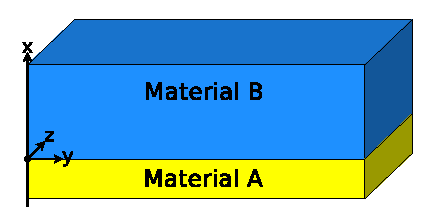
\includegraphics[width=10.0cm]{sketch}
\caption[Sketch]{A sketch of the system simulated in the script.}
\label{fig:sketch}
\end{center}
\end{figure}


\begin{figure}[!p]
\lstinputlisting[linerange=1-46]{spatially.py}
\caption{Part 1.}
\end{figure}

\begin{figure}[!p]
\lstinputlisting[linerange=47-94,firstnumber=47]{spatially.py}
\caption{Part 2.}
\end{figure}


\section{What Nmag5 cannot do, yet} \label{sec:missing_from_nmag5}
Here is a list of what is missing from Nmag5:
\begin{itemize}
\item It is not possible to run simulations where the applied field
  change continuously in time;
\item Simulate 1D and 2D systems (should be easy to fix);
\item Dynamic field dependency is not available, yet. This means that
  if you change the magnetization and probe the demag field, you will
  obtain an out-of-date demag field.
\end{itemize}

\end{document}
